%%%%%%%%%%%%%%%%%%%%%%%%%%%%%%%%%%%%%%%%%%%%%%%%%%%%%%%%%%%%%%%%%%%%%%%%%%%%%%%%
%2345678901234567890123456789012345678901234567890123456789012345678901234567890
%        1         2         3         4         5         6         7         8

\documentclass[letterpaper, 10 pt, conference]{ieeeconf}  % Comment this line out if you need a4paper

%\documentclass[a4paper, 10pt, conference]{ieeeconf}      % Use this line for a4 paper

\IEEEoverridecommandlockouts                              % This command is only needed if 
                                                          % you want to use the \thanks command

\overrideIEEEmargins                                      % Needed to meet printer requirements.

%In case you encounter the following error:
%Error 1010 The PDF file may be corrupt (unable to open PDF file) OR
%Error 1000 An error occurred while parsing a contents stream. Unable to analyze the PDF file.
%This is a known problem with pdfLaTeX conversion filter. The file cannot be opened with acrobat reader
%Please use one of the alternatives below to circumvent this error by uncommenting one or the other
%\pdfobjcompresslevel=0
%\pdfminorversion=4

% See the \addtolength command later in the file to balance the column lengths
% on the last page of the document

% The following packages can be found on http:\\www.ctan.org
%\usepackage{graphics} % for pdf, bitmapped graphics files
%\usepackage{epsfig} % for postscript graphics files
%\usepackage{mathptmx} % assumes new font selection scheme installed
%\usepackage{times} % assumes new font selection scheme installed
%\usepackage{amsmath} % assumes amsmath package installed
%\usepackage{amssymb}  % assumes amsmath package installed

\usepackage{cite}
\usepackage{amsmath}   % Required for align, matrices, and equation formatting
\usepackage{amssymb}   % Recommended for additional math symbols
\usepackage{bm}        % For bold symbols in equations
\usepackage{graphicx}  % Required if you include images
\usepackage{booktabs}   
\usepackage{caption}
\usepackage{subcaption} 
\usepackage{afterpage}
\usepackage{float}  

\title{\LARGE \bf
A 3-RRR Parallel Mechanism for Multi-DOF Ankle Rehabilitation 
}


% \author{Siyuan Zhang$^{1,}$\textsuperscript{*}, Yufei Zhang$^{1,2,}$\textsuperscript{*} and Junlin Lyu$^{1,}$\textsuperscript{*}% <-this % stops a space
% \thanks{*These author above contributed equally to this work.}% <-this % stops a space
% \thanks{$^{1}$Both in Mechanical Engineering,
%         Columbia University in the city of New York
%         {\tt\small}}%
% \thanks{$^{2}$Yufei Zhang is corresponding Author:
%         {\tt\small yz4917@columbia.edu}}%
% }
\author{Siyuan Zhang$^{1,}$\textsuperscript{*}, Yufei Zhang$^{1,}$\textsuperscript{*}, Junlin Lyu$^{1,}$\textsuperscript{*}, Sunil K. Agrawal$^{1, 2}$% <-this % stops a space
\thanks{*These authors contributed equally to this work.}% <-this % stops a space
\thanks{$^{1}$Department of Mechanical Engineering, 
        Columbia University in the City of New York.}%
\thanks{$^{2}$Prof.Sunil is the corresponding author: 
        {\tt\small sa3077@columbia.edu}}%
}

\begin{document}



\maketitle
\thispagestyle{empty}
\pagestyle{empty}


%%%%%%%%%%%%%%%%%%%%%%%%%%%%%%%%%%%%%%%%%%%%%%%%%%%%%%%%%%%%%%%%%%%%%%%%%%%%%%%%
\begin{abstract}

This paper introduces a wearable ankle rehabilitation device based on a 3-RRR spherical parallel mechanism (SPM) for multi-DOF ankle recovery. Designed for athletes and patients, it supports three rotational DOFs—pitch, yaw, and roll—to facilitate key ankle movements. The design ensures comfort with a simplified actuation layout and non-interference mechanisms. Kinematic modeling guides precise control, and preliminary tests show sufficient accuracy for rehabilitation. Future work will refine control and optimize patient-specific training to enhance clinical outcomes and user engagement.

\end{abstract}


%%%%%%%%%%%%%%%%%%%%%%%%%%%%%%%%%%%%%%%%%%%%%%%%%%%%%%%%%%%%%%%%%%%%%%%%%%%%%%%%
\section{INTRODUCTION}

Ankle injuries are prevalent, particularly among athletes and individuals recovering from surgery or neurological conditions. Effective rehabilitation is essential for restoring mobility, strength, and proprioception. However, conventional rehabilitation devices often impose only a few degree-of-freedom (DOF) constraints \cite{dong2021state}, limiting movement diversity and potentially prolonging recovery. While robotic platforms capable of multi-DOF motion have been explored, their bulk and complexity often hinder patient compliance and clinical integration.

The ankle joint can be approximated as a spherical joint, allowing for three rotational DOFs: pitch (plantarflexion), roll (eversion), and yaw (external rotation). Motivated by this biomechanical characteristic, we adopt a 3-RRR spherical parallel manipulator (SPM) to replicate natural ankle motion. SPMs offer stiffness, compactness, and precision, making them well-suited for joint rehabilitation. Now the 3-RRR SPM\cite{gosselin1989optimum} \cite{wu2019design} has been widely studied in robotics, finger rehabilitation\cite{he2021spindle}, and hip therapy\cite{sadeqi2017design}, but its application in wearable ankle rehabilitation remains largely unexplored.

The remainder of this paper is structured as follows: Section II details the mechanical design, Section III presents the kinematics, Section IV discusses the simulation and experimental results, section V for potential application, and Section VI concludes with the future work.

\section{MECHANISM DESIGN}

\subsection{Overview of the 3-RRR SPM}
A 3-RRR spherical parallel mechanism (SPM) consists of three identical limbs, each containing two revolute (R) joints that connect a base to a moving platform. The parallel arrangement allows for compact configurations that are well-suited to generating rotational motions around a common center of rotation. Although the 3-RRR architecture itself is well documented in robotics research~\cite{merlet2006parallel}, its application to wearable ankle rehabilitation has been limited. 

\begin{figure}[h]
    \centering
    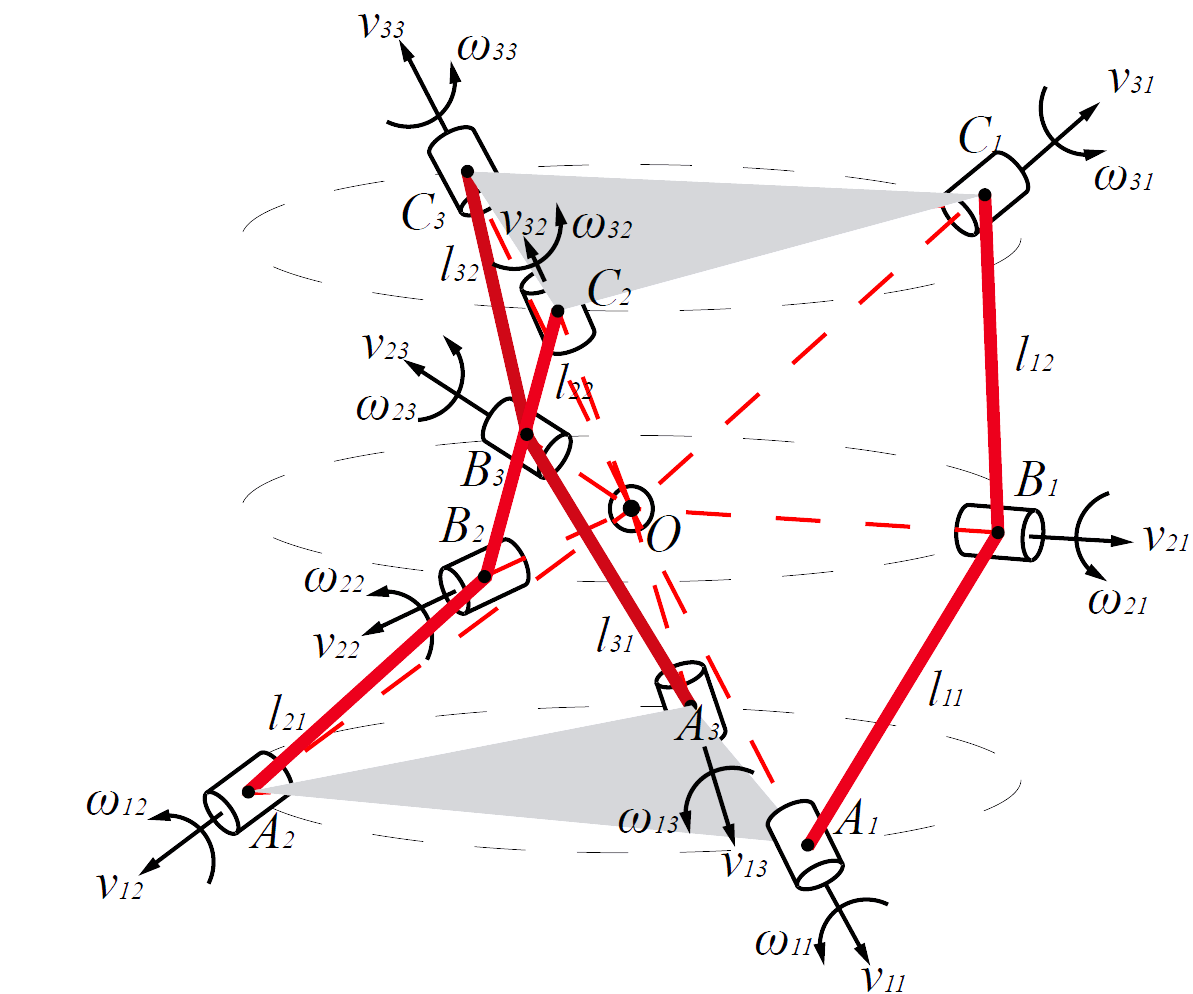
\includegraphics[width=0.8\linewidth]{SimplifiedModel.png}
    \caption{Schematic geometry model of the 3-RRR mechanism.}
    \label{fig:enter-label}
\end{figure}

Fig.~\ref{fig:enter-label} illustrates the schematic geometry model of the 3-RRR SPM, where the base is fixed, and the red lines represent the chains, each composed of 3 revolute joints and 2 connecting links. 

The proposed design consists of a ring-shaped base supporting three limbs, with a footplate as the moving platform. By adjusting limb lengths and angular offsets, the 3-RRR SPM enables three-DOF motion (pitch, yaw, roll), replicating natural ankle movements such as dorsiflexion/plantarflexion, inversion/eversion, and internal/external rotation. Although we are a spatial mechanism, our degrees of freedom are only three rotational degrees of freedom, so our order of screw system is 3, number of links is 8, number of joints is 9, freedom of the ith pair is 9, and the final computation gives mobility as 3. The parallel mechanism ensures its center of rotation aligns with the anatomical ankle joint to reduce motion discrepancies and discomfort.

Additionally, the wearable design presents engineering challenges but provides multi-DOF therapy in a portable format. This portability is particularly beneficial for athletes needing active rehabilitation and clinical environments with space limitations, making it a promising solution for dynamic ankle recovery and mobility enhancement.

\subsection{Design Considerations}
This device is designed for direct lower limb attachment, promoting daily use and better patient compliance. A wearable form factor requires both mechanical and ergonomic considerations:

\subsubsection{Compact Base Ring}
Custom-fitted to the calf for a secure yet non-restrictive fit, with adjustable straps for leg size variations.

\subsubsection{Non-Interference Mechanisms}
Low-profile limbs and joint housings minimize obstruction to nearby joints and ensure compatibility with footwear and braces.

\subsubsection{Device Modularity}
Interchangeable link segments and quick-release fasteners allow for size adjustments and rehabilitation stage customization, enhancing clinical utility.

\begin{figure}[H]
    \centering
    \begin{subfigure}{0.2\textwidth}
        \centering
        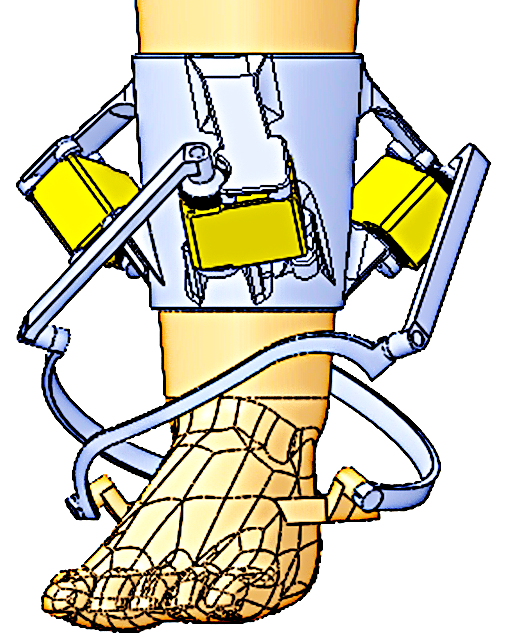
\includegraphics[width=\textwidth]{model.png}
        \caption{Rendered Model}
        \label{fig:fig1}
    \end{subfigure}
    \begin{subfigure}{0.2\textwidth}
        \centering
        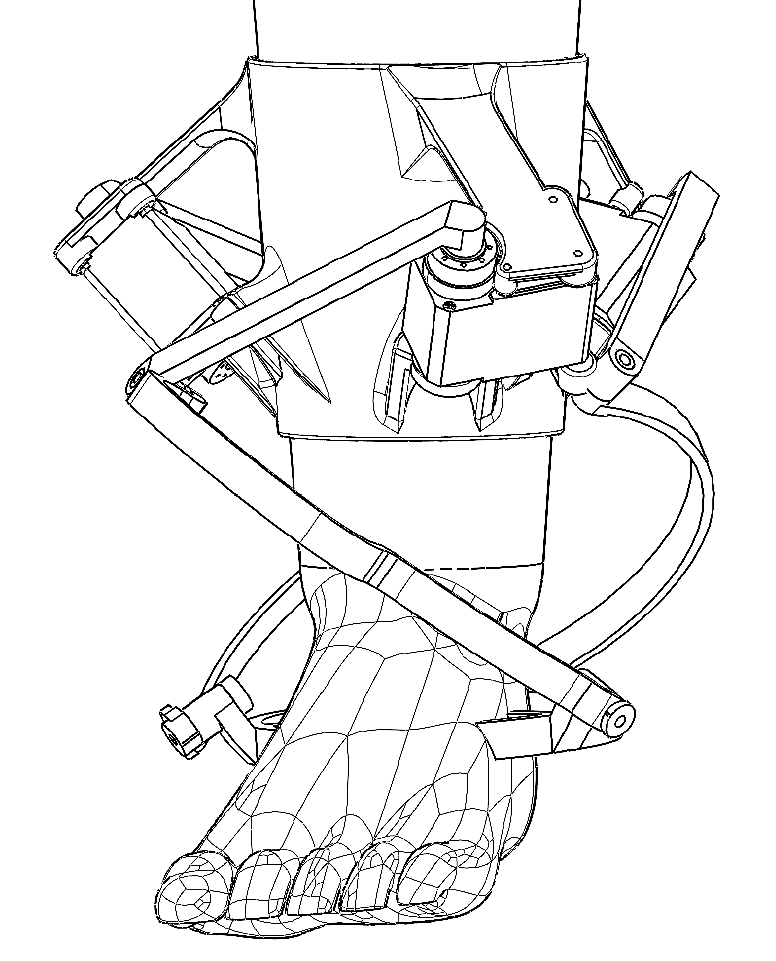
\includegraphics[width=\textwidth]{blackwhite.png}
        \caption{Line Drawing}
        \label{fig:fig2}
    \end{subfigure}
    \caption{SolidWorks CAD model}
    \label{fig:Solidworks Model}
\end{figure}  

\subsection{Detail Design}
To validate the design, a SolidWorks CAD model (Fig.~\ref{fig:Solidworks Model}) was developed, illustrating the base ring, limb connections, and footplate. The design was optimized for workspace, compactness, and portability, ensuring a balance between weight, power, and structural integrity to enhance patient comfort and rehabilitation effectiveness.

We 3D-printed the prototype to validate and demonstrate the design. Fig.~\ref{fig:combined2} below shows views of the device, highlighting its structure, fit, and support mechanisms.

\section{KINEMATIC MODELING}

\subsection{Comparison of Spherical and Cartesian Coordinates}
Kinematic modeling can be performed using spherical or Cartesian coordinate representations. Table~\ref{tab:coords} summarizes the key differences.

% \begin{table}[h]
% \centering
% \caption{Comparison of Spherical and Cartesian Coordinates}
% \label{tab:coords}
% \begin{tabular}{|c|c|c|c|}
% \hline
% \textbf{Aspect} & \textbf{Spherical $(\theta, \phi, R)$} & \textbf{Cartesian $(x, y, z)$} & \textbf{Benefit} \\
% \hline
% Variables & $3(\theta, \phi, R)$ & $3(x, y, z)$ & Less data \\
% Rotation Calculation & Matrix Multiplication & Direct angle transformation & Faster \\
% Forward Kinematics (FK) & Nonlinear system & Direct spherical mapping & Simpler \\
% Inverse Kinematics (IK) & Complex & Simple trigonometry & Easier to solve \\
% Computational Load & High & Low & More efficient \\
% \hline
% \end{tabular}
% \end{table}
\renewcommand{\arraystretch}{1.2} 

\begin{table*}[t]
\centering
\caption{Comparison of Spherical and Cartesian Coordinates}
\label{tab:coords}
\begin{tabular}{@{}lccc@{}}
\toprule
\textbf{Aspect} & \textbf{Spherical $(R, \psi, \phi)$} & \textbf{Cartesian $(x, y, z)$} & \textbf{Benefit} \\
\midrule
Variables & $3(R, \psi, \phi)$ & $3(x, y, z)$ & Less data \\
Rotation Calculation & Matrix Multiplication & Direct angle transformation & Faster \\
Forward Kinematics (FK) & Nonlinear system & Direct spherical mapping & Simpler \\
Inverse Kinematics (IK) & Complex & Simple trigonometry & Easier to solve \\
Computational Load & High & Low & More efficient \\
\bottomrule
\end{tabular}
\end{table*}
The spherical coordinate system simplifies motion parameterization while reducing data redundancy, making it particularly useful for modeling multi-DOF mechanisms such as the 3-RRR SPM.

\subsection{Transformation Between Coordinate Systems}
For a given point $C_i = (x, y, z)$, it can be expressed in spherical coordinates as:

\begin{equation}
(x, y, z) = (R \cos\psi \cos\phi, R \sin\psi \cos\phi, R \sin\phi)
\end{equation}

where:
\begin{itemize}
    \item $\psi$: Azimuth angle around the $z$-axis.
    \item $\phi$: Elevation angle measured from the $xy$-plane.
\end{itemize}

The position of a base point $A_i$ is defined as:

\begin{equation}
A_i = (R_A, \psi_A, \phi_A)
\end{equation}

Similarly, the position of a point in the end-effector frame is:

\begin{equation}
C_{i0} = (R_P, \psi_{Pi0}, \phi_{Pi0})
\end{equation}

\subsection{Rotation and Transformation Matrices}
The rotation matrix describing the transformation from the base frame to the ankle joint coordinate frame is given by:

\begin{equation}
R = R_z(\alpha) R_y(\beta) R_x(\gamma)
\end{equation}

Applying this rotation matrix to the initial end-effector coordinates $C_{i0}$:

\begin{equation}
C_i = R \cdot C_{i0}
\end{equation}

Transforming back to spherical coordinates:

\begin{align}
\psi_{Ci} &= \tan^{-1} \left( \frac{C_{iy}}{C_{ix}} \right) \\
\phi_{Ci} &= \sin^{-1} \left( \frac{C_{iz}}{R_C} \right)
\end{align}

\subsection{Inverse Kinematics}
The inverse kinematics problem is formulated by enforcing the link length constraints:

\begin{align}
\| B_i - A_i \| &= l_1 \\
\| C_i - B_i \| &= l_2
\end{align}

where $l_1$ and $l_2$ are the fixed link lengths. The distance between points $A_i$ and $C_i$ is given by:

\begin{equation}
d = \| C_i - A_i \|
\end{equation}

Solving for $\lambda$:

\begin{equation}
\lambda = \frac{l_1^2 - l_2^2 + d^2}{2d^2}
\end{equation}

The position of joint $B_i$ is calculated as:

\begin{equation}
B_i = A_i + \lambda (C_i - A_i) + \mu \frac{(C_i - A_i) \times N}{\|(C_i - A_i) \times N\|}
\end{equation}

where $N$ is the unit normal vector, and $\mu$ is determined using:

\begin{equation}
\mu = \sqrt{l_1^2 - \lambda^2 d^2}
\end{equation}

The joint angles $\theta_i$ are then obtained from:

\begin{equation}
\theta_i = \cos^{-1} \left( \frac{(B_i - A_i) \cdot u_i}{\|B_i - A_i\|} \right)
\end{equation}

where $u_i$ is the direction vector of the joint axis.

\subsection{Forward Kinematics}
The forward kinematics computation starts with the known active joint rotation angles $\theta_1, \theta_2, \theta_3$. Each base joint $A_i$ is parameterized in spherical coordinates:

\begin{equation}
A_i = (R_A, \psi_{Ai}, \phi_{Ai})
\end{equation}

The first link rotates by $\theta_i$, yielding the new joint position:

\begin{equation}
B_i = A_i + R_i(\theta_i) \cdot 
\begin{bmatrix}
l_1 \\ 0 \\ 0
\end{bmatrix}
\end{equation}

Since $C_i$ must be on a sphere centered at $B_i$ with radius $l_2$, the final position of $C_i$ is determined using an additional transformation matrix $R_{platform}$:

\begin{equation}
C_i = B_i + R_{platform} \cdot
\begin{bmatrix}
l_2 \\ 0 \\ 0
\end{bmatrix}
\end{equation}\section{Dynamic Modeling}
Let generalized coordinates be
$\mathbf{q}=[\theta_1,\theta_2,\theta_3,\alpha,\beta,\gamma]^T$. The closed‑chain constraints are written as $\mathbf{h}(\mathbf{q})=0$. The Lagrangian is
\begin{equation}
L=T-V,
\end{equation}
with
\begin{subequations}
\begin{align}
T&=\tfrac12\boldsymbol{\omega}^T I_P\boldsymbol{\omega}+\tfrac12\sum_{i=1}^3 I_{L,i}\dot{\theta}_i^2,\\
V&=m_Pgz_P+\sum_{i=1}^3 m_{i1} g z_{i1}+m_{i2} g z_{i2}.
\end{align}
\end{subequations}
Applying Lagrange's equations with constraint forces yields
\begin{equation}
\frac{d}{dt}\frac{\partial L}{\partial\dot{q}_j}-\frac{\partial L}{\partial q_j}=Q_j+\sum_{k}\lambda_k\frac{\partial h_k}{\partial q_j}.
\end{equation}
Eliminating multiplier $\lambda$ gives the reduced EOM:
\begin{equation}
M(\mathbf{q})\ddot{\mathbf{q}}+C(\mathbf{q},\dot{\mathbf{q}})\dot{\mathbf{q}}+G(\mathbf{q})=\boldsymbol{\tau}.
\end{equation}
Closed‑form expressions for $M$, $C$, and $G$ follow standard SPM dynamics (see \cite{Staicu2006}).
\section{Dynamics Modeling}

\subsection{Generalized Coordinates Definition}
Let the generalized coordinates be
\[
  \mathbf{q} = \begin{bmatrix}\theta_1\\\theta_2\\\theta_3\end{bmatrix},
\]
where \(\theta_i\) are the input angles of the 3‑RRR spherical parallel mechanism.

\subsection{Energy Expressions}

\paragraph{(1) Kinetic Energy \(T\):}
\[
  T = \frac{1}{2}\,\boldsymbol{\omega}^T I_P\,\boldsymbol{\omega}
      + \frac{1}{2}\sum_{i=1}^3 I_{\ell,i}\,\dot\theta_i^2,
\]
\begin{itemize}
  \item \(I_P\): inertia tensor of the platform.
  \item \(I_{\ell,i}\): inertia of the actuated links.
\end{itemize}

\paragraph{(2) Potential Energy \(V\):}
\[
  V = m_p\,g\,h_p(q)
      + \sum_{i=1}^3 \frac{1}{2}\,k_i\,\Delta\ell_i^2
      + \sum_{i=1}^3 m_s\,g\,h_s,
\]
\begin{itemize}
  \item \(m_p\): platform mass, \(h_p(q)\): platform height.
  \item \(k_i\): spring stiffness, 
        \(\Delta \ell_i = \|\mathbf{C}_i - \mathbf{A}_i\| - \ell_{0,i}\).
  \item \(m_s\): sliding unit mass, \(h_s\): constant height.
\end{itemize}

\subsection{Lagrangian Dynamics}
Define the Lagrangian
\[
  L = T - V.
\]
Applying Lagrange’s equations,
\[
  \frac{d}{dt}\biggl(\frac{\partial L}{\partial \dot{\mathbf{q}}}\biggr)
  \;-\;
  \frac{\partial L}{\partial \mathbf{q}}
  \;=\;
  \boldsymbol{\tau}.
\]

\subsection{Equations of Motion}
The resulting dynamics take the form
\[
  M(\mathbf{q})\,\ddot{\mathbf{q}}
  \;+\;
  C(\mathbf{q},\dot{\mathbf{q}})\,\dot{\mathbf{q}}
  \;+\;
  J_r^T\,\boldsymbol{\tau}_{\mathrm{spring}}
  \;+\;
  G_p(\mathbf{q})
  \;=\;
  \boldsymbol{\tau},
\]
where
\begin{itemize}
  \item \textbf{Inertia matrix:}
    \[
      M(\mathbf{q})
      = J_r^T\,I_P\,J_r \;+\; \mathrm{diag}(I_1,\,I_2,\,I_3).
    \]
  \item \textbf{Coriolis and centrifugal:}
    \[
      C(\mathbf{q},\dot{\mathbf{q}})\,\dot{\mathbf{q}}
      = J_r^T\,I_P\,\dot J_r\,\dot{\mathbf{q}}.
    \]
  \item \textbf{Gravity term:}
    \[
      G_p(\mathbf{q})
      = J_r^T\Bigl(m_p\,g\,\frac{\partial h_p}{\partial \mathbf{q}}\Bigr).
    \]
  \item \textbf{Spring-induced torque:}
    \[
      \boldsymbol{\tau}_{\mathrm{spring}}
      = \sum_{i=1}^3 \bigl(\mathbf{C}_i - O\bigr)
        \times \mathbf{F}_{\mathrm{spring},i},
    \]
    with
    \[
      \mathbf{F}_{\mathrm{spring},i}
      = -\,k_i\,\Delta\ell_i\,
        \frac{\mathbf{C}_i - \mathbf{A}_i}
             {\|\mathbf{C}_i - \mathbf{A}_i\|}.
    \]
\end{itemize}

\section{SIMULATION TO REALITY}

\subsection{Simulation Setup and Methodology}
A 3-DOF MATLAB simulation was conducted to validate the 3-RRR SPM for ankle rehabilitation, confirming its ability to achieve independent pitch, yaw, and roll, corresponding to key ankle plantarflexion, inversion, and external rotation.

The MATLAB simulation framework was developed to evaluate the system’s kinematic performance. The validation process consisted of:
\begin{enumerate}
    \item \textit{Forward Kinematics (FK) Analysis}
    \item \textit{Inverse Kinematics (IK) Validation}
    \item \textit{Motion Verification}
\end{enumerate}

A 3D simulation model (Fig.~\ref{fig:matlab_simulation}) was developed, with the red plate as the base and the blue plate as the end effector. The simulation validates the kinematic behavior by demonstrating that the end effector can achieve the desired roll, pitch, and yaw motions. Visual and numerical comparisons confirm its feasibility for rehabilitation applications.

\begin{figure}[h]
    \centering
    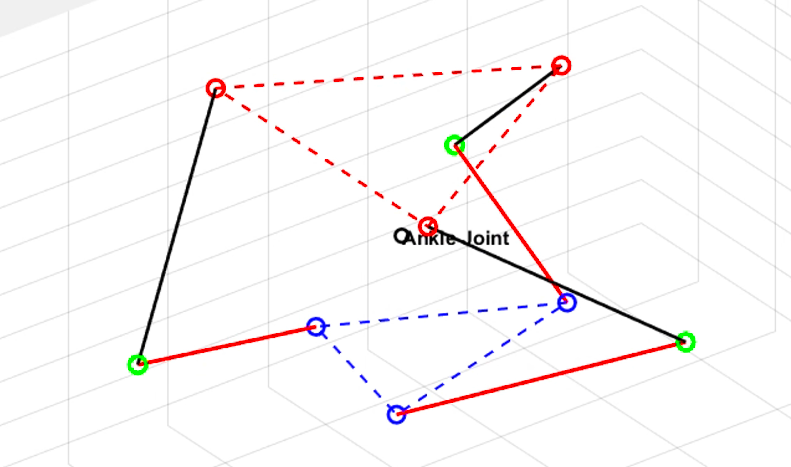
\includegraphics[width=0.4\textwidth]{simulation.png} 
    \caption{MATLAB simulation of the 3-RRR mechanism.}
    \label{fig:matlab_simulation}
\end{figure}

\subsection{Angle Error Analysis}
In order to verify that our kinematic model is calculated correctly, we let matlab calculate the error between our desired ankle rotation angle during simulation, and the actual rotation angle of the ankle joints driven by the three servo rotation angles obtained by IK solving, we used root mean square error (RMSE)\cite{chai2014root} and max error to validate the evaluation of our model. The following table summarizes the angle error analysis for the three axes (Yaw, Pitch, and Roll). The results show negligible errors, proving that there is no problem with our kinematic model.

\begin{table}[h]
    \centering
    \caption{Angle Error Analysis (Degrees)}
    \label{tab:angle_error}
    \begin{tabular}{lcc}
        \toprule
        \textbf{Angle Axis} & \textbf{RMSE (deg)} & \textbf{Max Error (deg)} \\
        \midrule
        Yaw   & 0.024142 & 0.035347 \\
        Pitch & 0.036591 & 0.047682 \\
        Roll  & 0.010390 & 0.025791 \\
        \bottomrule
    \end{tabular}
\end{table}

\subsection{Considerations for Physical Implementation}
While the MATLAB simulation provides preliminary validation, certain limitations must be addressed before transitioning to physical implementation:
\begin{enumerate}
    \item \textit{Friction and Backlash Effects}: The simulation assumes ideal conditions, ignoring mechanical losses that may affect joint actuation accuracy.
    \item \textit{Human Interaction Modeling}: External forces from the user’s foot are not modeled, potentially impacting movement execution and requiring adaptive control.
    \item \textit{Control System Latency}: The simulation lacks hardware constraints like sensor delays and motor response time, which must be addressed in real-world implementation.
\end{enumerate}

\subsection{Real World Model Establishment}
Based on the MATLAB simulation, we confirmed the mechanism's capability for certain motions and visualized them through SOLIDWORKS animation. 

To validate its real-world feasibility, we tested the 3D-printed model for roll, pitch, and yaw, confirming its alignment with the SOLIDWORKS animation and MATLAB simulation (Fig.~\ref{fig:combined2}). This successful sim-to-real validation allows us to proceed with motor integration and control implementation, advancing strategy toward a fully functional ankle rehabilitation system.
\begin{figure}[h]
    \centering
    \begin{subfigure}{0.15\textwidth}
        \centering
        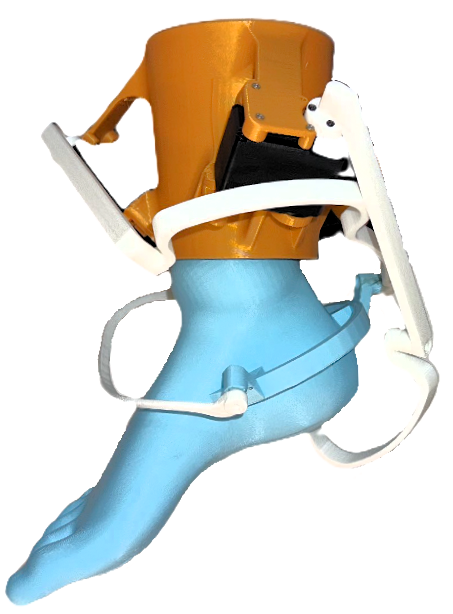
\includegraphics[width=\textwidth]{pitch.png}
        \caption{Pitch}
        \label{fig:fig1}
    \end{subfigure}
    \begin{subfigure}{0.15\textwidth}
        \centering
        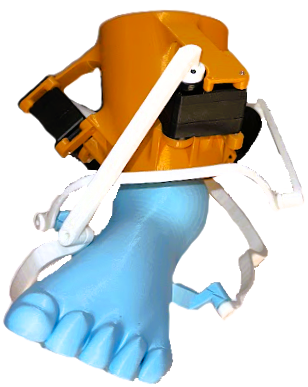
\includegraphics[width=\textwidth]{roll.png}
        \caption{Roll}
        \label{fig:fig2}
    \end{subfigure}
    \begin{subfigure}{0.16\textwidth}
        \centering
        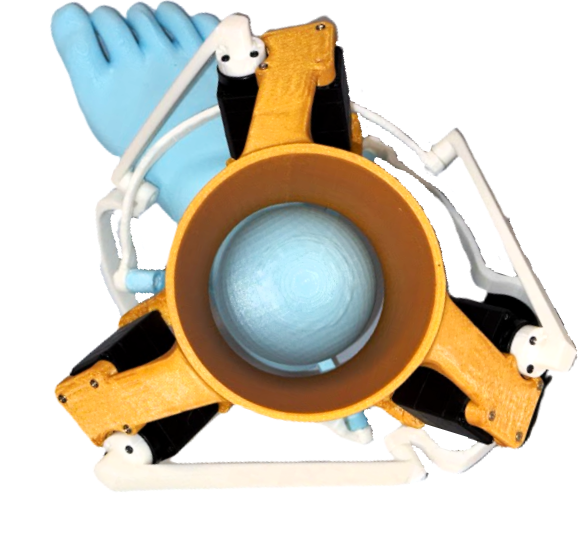
\includegraphics[width=\textwidth]{yaw.png}
        \caption{Yaw}
        \label{fig:fig3}        
    \end{subfigure}
    \caption{3D printed and view for the rehabilitation device.}
    \label{fig:combined2}
\end{figure}

\subsection{Future Experimental Validation}
The next phase will focus on hardware prototyping and experimental validation to refine the system’s performance. Key objectives include IMU-based motion tracking, force measurement for safety and compliance, and the implementation of adaptive control to accommodate user-specific movement patterns. These efforts will bridge the gap between simulation and real-world application, ensuring effective and safe rehabilitation.

\section{BROADER APPLICATIONS}

% Originally designed for ankle rehabilitation, the 3-RRR spherical parallel mechanism (SPM) offers a versatile platform for human motion assistance and industrial applications.

% In rehabilitation, it can be adapted into lower-limb exoskeletons\cite{exoskeleton_stroke} for patients with neurological disorders such as stroke, cerebral palsy, and spinal cord injuries. The mechanism's multi-DOF control allows for customized motion therapy, aiding in gait training, muscle recovery, and proprioception enhancement\cite{sale2012use}. It also has potential in sports rehabilitation, providing controlled resistance and guided movement to optimize recovery.

% Beyond medical applications, the high stiffness and precision of the 3-RRR SPM make it ideal for industrial automation. It can enhance robotic arms for precise alignment, be miniaturized for robotic end-effectors, or be applied to adaptive fixturing in CNC machining\cite{bakker2013active}. The ability to execute controlled pitch, yaw, and roll enables efficient workpiece positioning, improving manufacturing accuracy and flexibility.

Originally designed for ankle rehabilitation, the 3-RRR spherical parallel mechanism (SPM) is a versatile platform for human motion assistance and industrial applications.

In rehabilitation, it can be integrated into lower-limb exoskeletons\cite{exoskeleton_stroke} for patients with neurological disorders like stroke and spinal cord injuries. Its multi-DOF control supports customized motion therapy, aiding in gait training, muscle recovery, and proprioception enhancement\cite{sale2012use}. It also holds potential in sports rehabilitation by providing controlled resistance and guided movement.

Beyond medical applications, the 3-RRR SPM’s high stiffness and precision make it valuable for industrial automation. It can enhance robotic arms, be miniaturized for robotic end-effectors, or assist in adaptive fixturing for CNC machining\cite{bakker2013active}. Its controlled pitch, yaw, and roll improve workpiece positioning, enhancing manufacturing accuracy and flexibility.
\section{CONCLUSION AND FUTURE WORK}

In short, the study presents a wearable ankle rehabilitation device based on a 3-RRR SPM, enabling multi-DOF motion in a compact, portable form. Kinematic modeling and MATLAB simulations validate its feasibility for ankle recovery, confirming its ability to replicate key rehabilitation motions.

\begin{figure}[h]
    \centering
    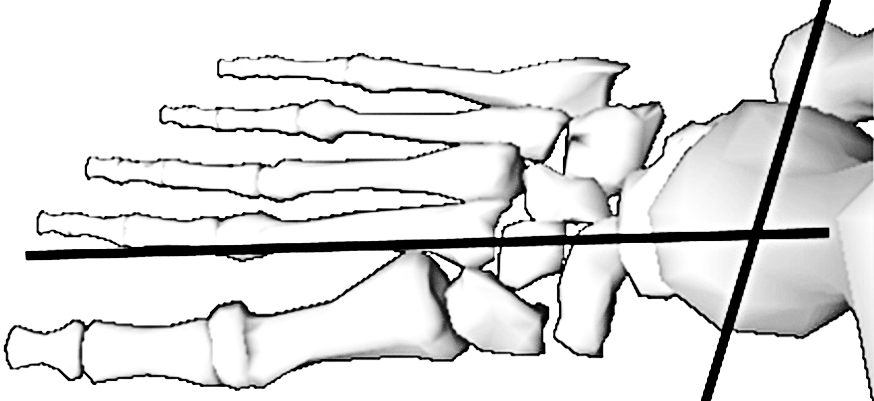
\includegraphics[width=0.5\linewidth]{ankle.png}
    \caption{Real Ankle\cite{brockett2016biomechanics}}
    \label{fig:real ankle}
\end{figure}

Beyond rehabilitation, the 3-RRR SPM could be adapted for assistive walking and running devices, benefiting patients with neuromuscular impairments or mobility limitations. By integrating real-time adaptive control and biomechanical feedback, it could support gait training, balance correction, and dynamic motion assistance. 

In previous calculations, the joint rotation angle was assumed to originate from a single point, which was also considered the center of the sphere. However, as illustrated in Fig.~\ref{fig:real ankle}, the actual movement of the ankle involves roll, pitch, and yaw about different points and different axes. Therefore, future design improvements will focus on enhancing ergonomic compatibility, with further testing conducted on human subjects. We will focus on the much correct model that fits the real ankle to be more realistic and suitable. 

In conclusion, the proposed system has the potential to advance rehabilitation and assistive robotics, ultimately enhancing human mobility and quality of life!

\addtolength{\textheight}{-12cm}   % This command serves to balance the column lengths
                                  % on the last page of the document manually. It shortens
                                  % the textheight of the last page by a suitable amount.
                                  % This command does not take effect until the next page
                                  % so it should come on the page before the last. Make
                                  % sure that you do not shorten the textheight too much.

%%%%%%%%%%%%%%%%%%%%%%%%%%%%%%%%%%%%%%%%%%%%%%%%%%%%%%%%%%%%%%%%%%%%%%%%%%%%%%%%



%%%%%%%%%%%%%%%%%%%%%%%%%%%%%%%%%%%%%%%%%%%%%%%%%%%%%%%%%%%%%%%%%%%%%%%%%%%%%%%%



%%%%%%%%%%%%%%%%%%%%%%%%%%%%%%%%%%%%%%%%%%%%%%%%%%%%%%%%%%%%%%%%%%%%%%%%%%%%%%%%
%%%%%%%%%%%%%%%%%%%%%%%%%%%%%%%%%%%%%%%%%%%%%%%%%%%%%%%%%%%%%%%%%%%%%%%%%%%%%%%%



\bibliographystyle{IEEEtran}  
\begin{thebibliography}{99}

\bibitem{gosselin1989optimum}
Gosselin, C. M., \& Angeles, J. (1989). The optimum kinematic design of a spherical three-degree-of-freedom parallel manipulator. \textit{Journal of Mechanisms, Transmissions, and Automation in Design}, 111(2), 202-207.

\bibitem{merlet2006parallel}
Merlet, J.-P. (2006). Jacobian, manipulability, condition number, and accuracy of parallel robots. \textit{The International Journal of Robotics Research}, 25(6), 557-571.

\bibitem{he2021spindle}
He, P., Kantu, N. T., Xu, B., Swami, C. P., Saleem, G. T., \& Kang, J. (2021). A novel 3-RRR spherical parallel instrument for daily living emulation (SPINDLE) for functional rehabilitation of patients with stroke. \textit{International Journal of Advanced Robotic Systems}, 18(3). \url{https://doi.org/10.1177/17298814211012325}

\bibitem{exoskeleton_stroke}
Dollar, A. M., \& Herr, H. (2008). Lower extremity exoskeletons and active orthoses: Challenges and state-of-the-art. \textit{IEEE Transactions on Robotics}, 24(1), 144-158.

\bibitem{sadeqi2017design}
Sadeqi, S., Bourgeois, S. P., Park, E. J., \& Arzanpour, S. (2017). Design and performance analysis of a 3-RRR spherical parallel manipulator for hip exoskeleton applications. \textit{Journal of Rehabilitation and Assistive Technologies Engineering}, 4, 2055668317697596. \url{10.1177/2055668317697596}

\bibitem{sale2012use}
Sale, P., Franceschini, M., Waldner, A., Hesse, S., et al. (2012). Use of the robot assisted gait therapy in rehabilitation of patients with stroke and spinal cord injury. \textit{European Journal of Physical and Rehabilitation Medicine}, 48(1), 111-121.

\bibitem{bakker2013active}
Bakker, O. J., Papastathis, T. N., Popov, A. A., \& Ratchev, S. M. (2013). Active fixturing: literature review and future research directions. \textit{International Journal of Production Research}, 51(11), 3171-3190.

\bibitem{wu2019design}
Wu, G., \& Bai, S. (2019). Design and kinematic analysis of a 3-RRR spherical parallel manipulator reconfigured with four-bar linkages. \textit{Robotics and Computer-Integrated Manufacturing}, 56, 55-65. \url{10.1016/j.rcim.2018.08.006}

\bibitem{dong2021state}
Dong, M., Zhou, Y., Li, J., Rong, X., Fan, W., Zhou, X., \& Kong, Y. (2021). State of the art in parallel ankle rehabilitation robot: a systematic review. \textit{Journal of NeuroEngineering and Rehabilitation}, 18(1). \url{10.1186/s12984-021-00845-z}

\bibitem{chai2014root}
Chai, T., \& Draxler, R. R. (2014). Root mean square error (RMSE) or mean absolute error (MAE). \textit{Geoscientific Model Development Discussions}, 7(1), 1525-1534.

\bibitem{james2024rehabilitation}
James, S. G. (1995). Rehabilitation of the foot and ankle. \textit{Online resource}. Available at: \url{https://cir.nii.ac.jp/crid/1130000793859809792}

\bibitem{brockett2016biomechanics}
Brockett, C. L., \& Chapman, G. J. (2016). Biomechanics of the ankle. \textit{Orthopaedics and Trauma}, 30(3), 232-238. \url{10.1016/j.mporth.2016.04.015}

\end{thebibliography}


% \bibitem{c1} G. O. Young, ÒSynthetic structure of industrial plastics (Book style with paper title and editor),Ó 	in Plastics, 2nd ed. vol. 3, J. Peters, Ed.  New York: McGraw-Hill, 1964, pp. 15Ð64.
% \bibitem{c2} W.-K. Chen, Linear Networks and Systems (Book style).	Belmont, CA: Wadsworth, 1993, pp. 123Ð135.
% \bibitem{c3} H. Poor, An Introduction to Signal Detection and Estimation.   New York: Springer-Verlag, 1985, ch. 4.
% \bibitem{c4} B. Smith, ÒAn approach to graphs of linear forms (Unpublished work style),Ó unpublished.
% \bibitem{c5} E. H. Miller, ÒA note on reflector arrays (Periodical styleÑAccepted for publication),Ó IEEE Trans. Antennas Propagat., to be publised.
% \bibitem{c6} J. Wang, ÒFundamentals of erbium-doped fiber amplifiers arrays (Periodical styleÑSubmitted for publication),Ó IEEE J. Quantum Electron., submitted for publication.
% \bibitem{c7} C. J. Kaufman, Rocky Mountain Research Lab., Boulder, CO, private communication, May 1995.
% \bibitem{c8} Y. Yorozu, M. Hirano, K. Oka, and Y. Tagawa, ÒElectron spectroscopy studies on magneto-optical media and plastic substrate interfaces(Translation Journals style),Ó IEEE Transl. J. Magn.Jpn., vol. 2, Aug. 1987, pp. 740Ð741 [Dig. 9th Annu. Conf. Magnetics Japan, 1982, p. 301].
% \bibitem{c9} M. Young, The Techincal Writers Handbook.  Mill Valley, CA: University Science, 1989.
% \bibitem{c10} J. U. Duncombe, ÒInfrared navigationÑPart I: An assessment of feasibility (Periodical style),Ó IEEE Trans. Electron Devices, vol. ED-11, pp. 34Ð39, Jan. 1959.
% \bibitem{c11} S. Chen, B. Mulgrew, and P. M. Grant, ÒA clustering technique for digital communications channel equalization using radial basis function networks,Ó IEEE Trans. Neural Networks, vol. 4, pp. 570Ð578, July 1993.
% \bibitem{c12} R. W. Lucky, ÒAutomatic equalization for digital communication,Ó Bell Syst. Tech. J., vol. 44, no. 4, pp. 547Ð588, Apr. 1965.
% \bibitem{c13} S. P. Bingulac, ÒOn the compatibility of adaptive controllers (Published Conference Proceedings style),Ó in Proc. 4th Annu. Allerton Conf. Circuits and Systems Theory, New York, 1994, pp. 8Ð16.
% \bibitem{c14} G. R. Faulhaber, ÒDesign of service systems with priority reservation,Ó in Conf. Rec. 1995 IEEE Int. Conf. Communications, pp. 3Ð8.
% \bibitem{c15} W. D. Doyle, ÒMagnetization reversal in films with biaxial anisotropy,Ó in 1987 Proc. INTERMAG Conf., pp. 2.2-1Ð2.2-6.
% \bibitem{c16} G. W. Juette and L. E. Zeffanella, ÒRadio noise currents n short sections on bundle conductors (Presented Conference Paper style),Ó presented at the IEEE Summer power Meeting, Dallas, TX, June 22Ð27, 1990, Paper 90 SM 690-0 PWRS.
% \bibitem{c17} J. G. Kreifeldt, ÒAn analysis of surface-detected EMG as an amplitude-modulated noise,Ó presented at the 1989 Int. Conf. Medicine and Biological Engineering, Chicago, IL.
% \bibitem{c18} J. Williams, ÒNarrow-band analyzer (Thesis or Dissertation style),Ó Ph.D. dissertation, Dept. Elect. Eng., Harvard Univ., Cambridge, MA, 1993. 
% \bibitem{c19} N. Kawasaki, ÒParametric study of thermal and chemical nonequilibrium nozzle flow,Ó M.S. thesis, Dept. Electron. Eng., Osaka Univ., Osaka, Japan, 1993.
% \bibitem{c20} J. P. Wilkinson, ÒNonlinear resonant circuit devices (Patent style),Ó U.S. Patent 3 624 12, July 16, 1990. 






% \end{thebibliography}




\end{document}
